% This is LLNCS.DEM the demonstration file of
% the LaTeX macro package from Springer-Verlag
% for Lecture Notes in Computer Science,
% version 2.4 for LaTeX2e as of 16. April 2010
%
\documentclass{llncs}
%
\usepackage{makeidx}  % allows for indexgeneration
\usepackage{graphicx}
\usepackage{color}
\graphicspath{{figs/}} 	
\usepackage{array}	
\usepackage{multirow}
		
	
%
\begin{document}
%
\frontmatter          % for the preliminaries
%
\pagestyle{headings}  % switches on printing of running heads
\addtocmark{Hamiltonian Mechanics} % additional mark in the TOC
%

%
\mainmatter              % start of the contributions
%
\title{A Deep Learning method for Classification of EEG data Based on Motor Imagery }
%
\titlerunning{Hamiltonian Mechanics}  % abbreviated title (for running head)
%                                     also used for the TOC unless
%                                     \toctitle is used
%
\author{Xiu An\inst{1} \and Deping Kuang\inst{1} \and Xiaojiao Guo\inst{1} \and Yilu Zhao\inst{1}
 \and  Lianghua He\inst{1}}
%
\authorrunning{Ivar Ekeland et al.} % abbreviated author list (for running head)
%
%%%% list of authors for the TOC (use if author list has to be modified)
\tocauthor{Ivar Ekeland, Roger Temam, Jeffrey Dean, David Grove,
Craig Chambers, Kim B. Bruce, and Elisa Bertino}
%
\institute{The Key Laboratory of Embedded System and Service Computing, Ministry of Education,
Tongji University, Shanghai 201804, China
,\\
Department of Computer Science and Technology, Tongji University, Shanghai 201804, China,\\
\email{anxiuaijia88@sina.cn}}
\maketitle              % typeset the title of the contribution

\begin{abstract}
Effectively extracting EEG data features is the key point in Brain Computer Interface technology. In this paper, aiming at classifying EEG data based on Motor Imagery task, Deep Learning (DL) algorithm was applied. For the classification of left and right hand motor imagery, firstly, based on certain single channel, a weak classifier was trained by deep belief net (DBN); then borrow the idea of Ada-boost algorithm to combine the trained weak classifiers as a more powerful one. During the process of constructing DBN structure, we stacked many RBMs (Restrict Boltzmann Machine) on top of each other by setting the hidden layer of the bottom layer RBM as the visible layer of the next RBM, and Contrastive Divergence (CD) algorithm was also exploited to train multilayered DBN effectively. The performance of the proposed DBN was tested with different combinations of hidden units and hidden layers on multiple subjects, the experimental results showed that the proposed method performs better with 8 hidden layers. The average recognition accuracy rate of DBN with 8 hidden layers is 81\%, and the highest accuracy can reach to 95\% for certain cases.
\keywords{Deep Learning, Motor Imagery, EEG, Brain-computer interface, Ada-boost}
\end{abstract}
%
\section{Introduction}
%
Brain-computer interface is a communication control system without depending on the normal output pathways that composed by brain, peripheral nerve and muscles, that can transfer brain information and realize control by using computer or electrical device to analyze the brain activities under specific task\cite{1}. In the current BCI technology and knowledge development, the brain-computer interface researchers have tried to create numerous BCI to enhance the function of body and made good progress in the field of human-computer interaction and machine intelligence. In recent studies on Motor Imagery, there are many ways to classify different kinds of MI\cite{9}. Studies had shown that the performance of the proposed BCI using feature extracted by MSCE yielded a promising inter-subject validation accuracy of over 90\% in classifying  with K-Nearest Neighbor(K-NN) and Support Vector Machine(SVM)\cite{1}. The studies conducted by Like’s group demonstrated that combining multi-scale filters and Principal Component Analysis (PCA) to enhance the classification performance in identifying EEG signals works and achieve a classification accuracy of 91.13\% which might enhance the performance of a BCI system in signal recognition\cite{2}. 


A lot of studies have done by Shang-Lin Wu and his follows indicates that using the common spatial pattern(CSP) for feature extraction from EEG and the linear discriminant analysis(LDA) for motor imagery classification obtained an average classification accuracy of 80\% for two subjects using only 9 channels, without any feature selection\cite{4}. Additionally, Yohimbe et al. proposed bimodal approach that using near infrared spectroscopy (NIRS) simultaneously with EEG to measure the hemodynamic fluctuations in the brain during stimulation with steady-state visual evoked potentials (SSVEP) made the wrong classification for 9 classes for 13 subjects’ decrease\cite{7}. Most of the existing methods of average classification accuracy of 80\% for two subjects using only 9 channels, without any feature selection\cite{4}.Most of the existing methods of analysis using whole channels to classify and the extracted feature could not achieve the desired recognition rate.


Deep Learning is a new field in itself in the machine learning whose motivation is to simulate the human brain’s mechanism to explain the data by the composition of multiple non-linear transformations of the data, with the goal of obtain more abstract and ultimately more useful representation\cite{3}\cite{5}. Despite the success of DBN, its application in Electroencephalogram (EEG)-based Brain Computer Interaction (BCI) is still rare. The main difficulty is the enormously high feature dimensionality spanning EEG channel, frequency, and time\cite{10}. Thus, it is necessary to develop more effective feature extraction method and technique for improving the accuracy of classification. Deep Learning algorithm has shown superior learning and classification performance in fields such as computer vision, natural language processing and other areas for its excellent feature extraction capabilities except the field of EEG data analysis\cite{15}. 

In this paper, we proposed a classify method based on deep learning with Ada-boost algorithm. Using this method, the misclassification rate of EEG signals decreased even using fewer channels. Firstly, we constructed the DBN by many RBMs and each RBM can be regarded as a two layers of neurons: a visible layer and a hidden layer. Each neuron is no connection between neurons of the same layer. And then we trained the RBM greedily and unsupervised layer by layer, during this period, CD algorithm was applied to optimize the whole performance of the trained model. For the training of weak classifier, we used single channel data of each subject and adopted the idea of Ada-boost to combine weak classifier. Finally, we got the powerful classifier that makes full use of all information. 


The sections below are our learning method and experiments. Section 2 mainly describes the theory of DBN and Section 3 presents our experimental results on MI EEG dataset.


\section{Method}

%
\subsection{Theory of Deep Learning}
%
Deep learning algorithm focus on learning multiple levels of representation of raw data automatically, using a deep architecture which composed of many hidden layers. This algorithm automatically extracts the high-level features necessary for classification which involving more meaningful information that hierarchically depends on other features, in other words, it learns its own low level representation from raw data and then build representations that associate with those low level representations and successively repeat the same procedure for higher levels. Here we use DBN model which formed by a plurality of RBM, each RBM is trained greedily and unsupervised\cite{5}.


An RBM has a single layer of hidden layer that are disconnected with the units in the same layer and have undirected, symmetrical connections to the units in the visible layer which makes it easy to compute the conditional probabilities. In an RBM, we can use the difference between two correlations of the output and input of the RBM that ensure the layer parameters to achieve optimal after training. The key issue of training the RBM is to get generative weights. As shown in Fig.\ref{fig:1}, $W$ represents the weights between visible and hidden layers, $b$, $c$ correspond to the bias of visual and hidden layer respectively \cite{3}.


The type of RBM we employed in this work is Gaussian RBMs which use real-valued visible units for training the first layer of the DBNs. Fig. \ref{fig:1} shows the structure of the RBM:
\begin{figure}[!htbp]
	\centering
		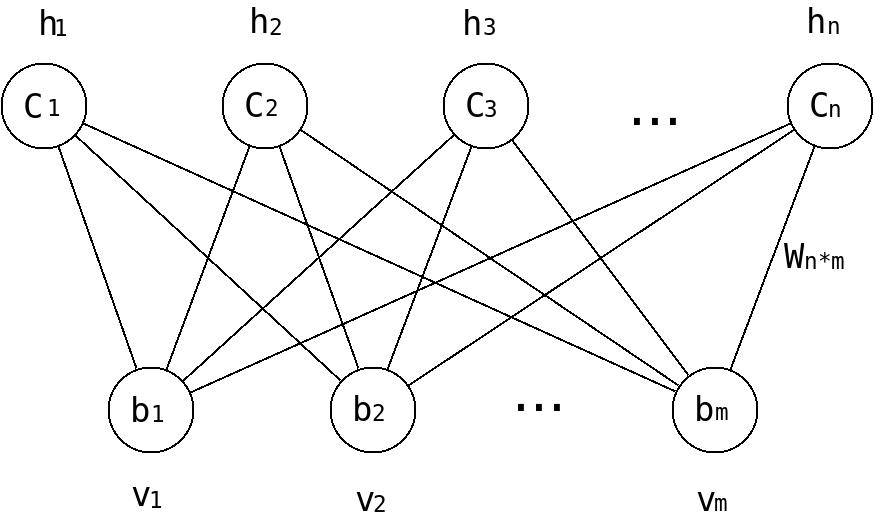
\includegraphics[scale=0.23]{figs/kdp1.jpeg}
		\caption{Strcture of RBM}  
    	\label{fig:1}
\end{figure}


\subsection{Classification of MI based on Deep Belief Net}
Now, let $v$ represent the feature vector containing only one channel features. An RBM defines a joint distribution on it, regard as the visible units in DBN and $h$, the hidden units as follow format\cite{13}
\begin{equation}
 p(v)=\frac{\sum_he^{-E(v,h)}}{\sum_u\sum_ge^{-E(u,g)}}
\end{equation}
Where $E$ is the energy function defined as
\begin{equation}
  E(v,h)=-\sum_{i \in visible}a_iv_i-
  \sum_{j \in hidden}b_jh_j-\sum_{i,j}v_ih_j\omega_{ij}
\end{equation}


Where $v_i$,$h_i$ are the binary states if visible unit $i$ and hidden unit $j$,$a_i$,$b_j$ are their biases and $w_{ij}$ is the weight between them. The network assigns a probability to every possible pair of a visible and a hidden vector via this energy function:
\begin{equation}
  P(v,h)=\frac{1}{Z}\exp(-E(v,h))
\end{equation}
Where the “partition function” $Z$ represents by
\begin{equation}
 Z=\sum_{v,h}e^{-E(v,h)}
\end{equation}


The probability that the network assigns to a training data can be optimized by adjusting the
weights and biases to lower the energy of it. The derivative of the log probability of a training vector with respect to a weight calculated as follow:
\begin{equation}
\frac{\partial \log p(v)}{\partial \omega_{ij}}
=\frac{\sum_{v \in D}\partial \log p(v)}{\partial \omega_{ij}}
=E_{data}\frac{\partial E(v,h)}{\partial \omega_{ij}}-
E_{model}\frac{\partial E(u,g)}{\partial \omega_{ij}}
\end{equation}
Where the first item is the expectation of $\frac{\partial E(v,h)}{\partial \omega_{ij}}$ respond to the training set D and the hidden variables are sampled according to the conditional distribution of the dataset on $p(h|v)$, given a randomly selected training sample, $v$, the binary state,$h_j$, of each hidden unit, $j$, is set to 1 with probability
\begin{equation}
 p(h_j=1|v)=\sigma(\sum_{i}v_i\omega_{ij}+b_j)
\end{equation}
Where $\sigma(x)$ is the logistic sigmoid function ${1}/{(1+exp{(-x))}}$.$v_ih_j$ is then an unbiased sample.


For no direct connections between visible units in an RBM, it is also the way to get unbiased sample of the visible unit similar as hidden unit, given a hidden vector
\begin{equation}
 p(v_i=1|h)=\sigma(\sum_{j}h_j\omega_{ij}+a_i)
\end{equation}

                                          
To construct a DBN, we stack many RBMs on top of each other by setting the hidden layer of the bottom layer RBM as the visible layer of the next RBM. An algorithm called Contrastive Divergence (CD) is applied to train multilayered DBN effectively\cite{5}.


For training an RBM classifier, the joint distribution of data and class labels, the visible vector is concatenated with binary vector of class labels. The energy function becomes:
\begin{equation}
 E(v,l,h)=-\sum_i a_iv_i - \sum_j b_jh_j - \sum_{i,j} \omega_{ij} - \sum_y c_yl_y -\sum_{y,j} \omega_{yj}h_jl_y
\end{equation}
Where $l$ is the binary class label and $\omega_{yj}$ is the weights between hidden and label units.


A RBM can be also understood as a two layers of neurons: a visible layer and a hidden layer. Each neuron is no connection between neurons of the same layer. For training DBN we feed features as input and labels are applied after pre-training.


\subsection{Boost of the single channel Deep Belief Net}
Based on the former test performance of the single channel, we adopt the idea of Ada-boost algorithm\cite{8} that combine the weak classifier to one more powerful classifier\cite{19}\cite{20}. Here we choose the channel C3, C4, Fc4 as the meta data and the combination tactics to boost each weak classifiers refer to follow\cite{15}\cite{16}:
\begin{equation}
M_k(X)=\sum_{k=1}^{k} c_kf_k(X)
\end{equation}                                                                           
Where $c_k$ is the estimated coefficient for each DBN model, and each DBN model produces a discrete classification for input data\cite{17}.


The whole structure of our model based on DBN shows in Fig.2 as follow:
\begin{figure}[!htbp]
	\centering 
		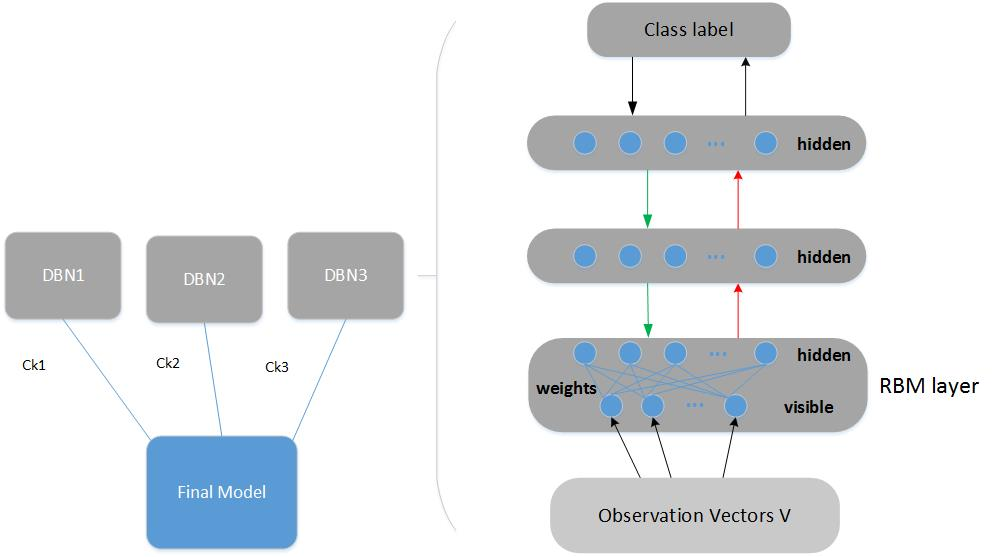
\includegraphics[scale=0.36]{figs/ax11.jpg}
		\caption{Structure of the final model} 
    	\label{fig:2}
\end{figure}


\section{Experiment}
\subsection{Experimental data}
The experimental data was collected from 4 subjects, all of them are students, male and without brain disease history. We selected 60 trials as sample for analysis for each subject that is to take 30 trials left-hand imagination EEG data and 30 right ones. Fig.3 shows the way we got the final data which contained 7s data, of which the search adopted the data from 3s to 7s. Particularly, the input to DBN were single channel of each subject whose sample rate is 250HZ/s and each of them contained 4s data, which means that each of them have 1000 sample points. 


For the EEG data, we did de-noising processing and filtering. As for de-noising processing, the main work is to remove noise such as Electro-Oculogram (EOG) as well as separated the data according to the channel. The EOG is removed by the Neuroscan software. And for the filtering work, this paper mainly analyzes the frequency band of 8-30Hz. So an elliptic filter was designed, with band-pass from 8 to 30Hz.And then converted the time domain data to frequency domain data via FFT(Fast Fourier Transformation) algorithm, on which employ normalization method to normalized the data between 0.2 to 0.8.  
\begin{figure}[!htbp]
	\centering  
		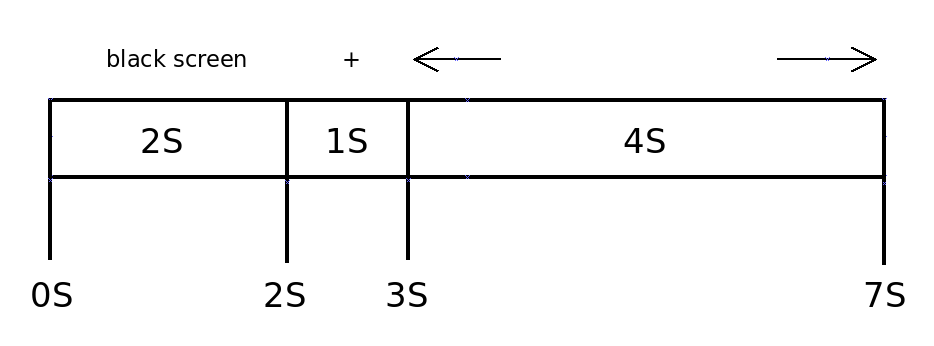
\includegraphics[scale=0.25]{figs/ax2.png}
		\caption{Experiment time distribution for one trial}
    	\label{fig:3}
\end{figure}

\subsection{Test on Combine of the single channel}
For each subject we select 20 trials as the train set from the total data with the remaining data to be the test samples from each channel. The weights were randomly initialized and the turning parameters were set as: learning rate for weight and biases = 0.07, momentum = 0.5 and weight decay = 0.002. After pre-training, the labels are concatenated with the last layer of DBN, so that the trained network can classify the left MI and the right MI.


First, we trained and tested for four to sixteen layers for each channel of every subject. Then we did the test that combine the weak classifier trained by each single channel as the idea of Ada-boost, here we select the channel which worked well in the former experiment, and follow the common trend of every subject. Finally, we adopt the parameter  according to the classification accurate of every individual channel which was tested before. The results for eight layers worked better than others and the performance of nine and ten or more layers were very similar. In the paper we have not shown results for all of the layers due to space limitations. Table \ref{tab1} shows the result of the classification performance with 7,8, 9, 10 layers respectively and the result shows that the average recognition rate of DBN with 8 hidden layers is 0.81 which is higher than others.


The result for every subject with different hidden layers lists in Table \ref{tab1} and the number represent the recognition accuracy rate:
\begin{table}
\caption{Performance of DBN with different layers}
\label{tab1}
\begin{center}
\begin{tabular}{|c|c|c|c|c|}
\hline
\multirow{2}{*}{Subjects}	& \multicolumn{4}{c|}{DBN}  \\
\cline{2-5}\rule{0pt}{12pt}
			 	& 7 hidden layers & 8 hidden layers & 9 hidden layers	&  10 hidden layers \\
\hline \rule{0pt}{12pt}
SHY				& 73\%		   & 85\%    &    83\%   &    80\% \\
XB				& 56\%		   & 65\%    &    59\%   &    58\% \\
ZJH				& 44\%	   	   & 77\%    &    78\%   &    74\% \\
WDM				& 82\%	   	   & 95\%    &    94\%   &    96\% \\[2pt]
\hline
\end{tabular}
\end{center}
\end{table}


Then we did the test for the different combination of hidden units, the result shows that there's no obvious effect on the performance. Table \ref{tab2} shows the final performance of the recognition rate of all cases and the number in table represent recognition accuracy rate:
\begin{table}
\caption{Performance of DBN with different hidden nodes}
\label{tab2}
\begin{center}
\begin{tabular}{|c|c|c|c|c|c|c|}
\hline
\multirow{5}{*}{Subjects}	& \multicolumn{6}{c|}{DBN\_8 layers}  \\
\cline{2-7}\rule{0pt}{12pt}
			 	& 2000-800- & 3000-1800- & 4000-1100-	&  5000-2100- & 6000-3100- & 8000-2100- \\
			 	& 700-600- & 1700-1600- & 1200-1300-	&  2200-2300- & 3200-3300- & 2200-2300- \\
			 	& 500-300- & 1500-1300- & 1400-1500-	&  2400-2500- & 3400-3500- & 2400-2500- \\
			 	& 200-900 & 1200-900 & 1600-900	&  2600-900 & 3600-1900 & 2600-1900- \\
\hline \rule{0pt}{12pt}
SHY				& 83\%		   & 84\%    &    84\%   &    85\% & 84\% & 85\% \\
XB				& 65\%		   & 66\%    &    65\%   &    65\% & 65\% & 64\%\\
ZJH				& 73\%	   	   & 75\%    &    77\%   &    77\% & 75\% & 74\%\\
WDM				& 96\%	   	   & 94\%    &    93\%   &    95\% & 95\% & 95\%\\[2pt]
\hline
\end{tabular}
\end{center}
\end{table}



\subsection{Experiment on time series}
We divided our experimental data by time segments, and each section contains 1s as data to be classified. Fig.4 presents the performance of classification with different subjects. From the figure we can see that the average recognition rate of first 2 seconds can reach 83\%, while the last 2 seconds is lower, we can explain that at the beginning of the experiment the subjects can preferably focus on the motor imagery experiment, but with the passage of time, the subjects may get absent-minded which would affect the validity of the experimental data, and finally leads to the low recognition accuracy. 
\begin{figure}[!htbp]
	\centering
		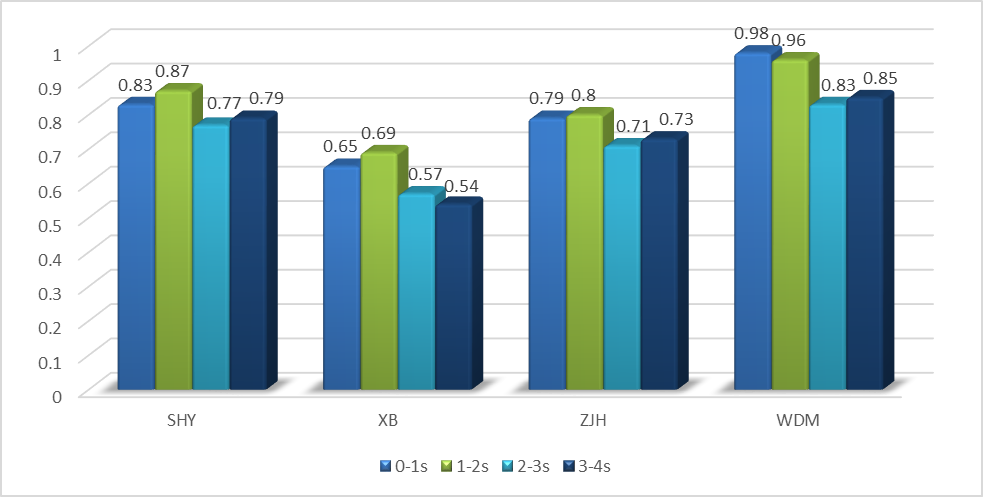
\includegraphics[scale=0.55]{figs/ax3.png}
		
		\caption{Classification accuracy of time series}  
    	\label{fig:4}
\end{figure}


\section{Conclusion}
In this paper, we proposed a DBN classifier for the classification of MI pattern. In our research, we found that the DBN model with 8 hidden layers has a better recognition performance through multiple cross-validation experiments. We also did the test on different combination of hidden units, and found that the number of nodes had no obvious effect on the performance of classification. The experimental results showed that Deep Learning algorithm performs effectively on the task of classification with MI data. And the experimental results of time series show that the performance of classification depends on concentration of the subjects, for the accuracy rate is affected greatly by the status of the subject. Our study suggests that DBN has great potential to be a powerful tool for the BCI research. 


For the next stage, we’ll try to employ this algorithm into classification of Multi-class based on EEG data, and merge more channels in order to take full use of the EEG data information to achieve better recognition results.



%
% ---- Bibliography ----
%
\begin{thebibliography}{}
%
\bibitem{1}
Reza, K., Chai, Q.:
A Brain-Computer Interface for classifying EEG correlates of chronic mental stress.
Proceedings of International Joint Conference on Neural Networks. 757--762 (2011)

\bibitem{2}
Li, K., Rui, Q.:
Classification of EEG Signals by Multi-Scale  Filtering and PCA.
Intelligent Computing and Intelligent Systems, 2009. ICIS 2009. IEEE International Conference on. 362--366 (2009)

\bibitem{3}
Gorge, H., S, O.:
A fast learning algorithm for deep belief nets.
Neural Computation. 1527--1554 (2006)

\bibitem{4}
Wu, S., Wu, W.:
Common Spatial Pattern and Linear Discriminant Analysis for Motor Imagery Classification.
Computational Intelligence, Cognitive Algorithms, Mind, and Brain (CCMB), 2013 IEEE Symposium on. 146--151 (2013)


\bibitem{5}
Yoshua, B., Pascal, L.:
Greedy layer-wise training of deep networks.
NIPS. (2006)

\bibitem{6}
Jarrett, K., Kavukcuoglu, K.:
What is the best ¨C  stage architecture for object recognition.
ICCV. (2009)

\bibitem{7}
Tomita, Y., Mitsukura, Y.:
Hemodynamic characteristics for improvement of EEG-BCI performance.
Human System Interaction (HSI), 2013 The 6th International Conference on. 495--500 (2013)

\bibitem{8}
Hancock, T., Mamitsuka, H.:
Boosted Network Classifiers for Local Feature Selection.
IEEE TRANSACTIONS ON NEURAL NETWORKS AND LEARNING SYSTEMS. 1767--1778 (2012)

\bibitem{9}
Plamen, D., Jesse, S.:
Classification of Imagined Motor Tasks for BCI.
Region 5 Conference, 2008 IEEE. 1--6 (2008)

\bibitem{10}
Karl, J.:
Characterizing  Functional Asymmetries with Brain Mapping.
The MIT Press. 161--186 (2003)

\bibitem{11}
Guger, C., Schlogl, A.:
Rapid prototyping of an EEG-based brain computer interface (BCI).
IEEE Trans. on Neural Systems and Rehabilitation Engineering. 49--58 (2001)

\bibitem{12}
Wolpaw, J., Birbaumer, N.:
Brian-computer interfaces for communication and control.
Clinical Neurophysiology. 767--791 (2002)

\bibitem{13}
Bengio, Y., Lecun, Y.:
Scaling learning algorithms towards AI.
Large-Scale Kernel Machines. 1--34 (2007)

\bibitem{14}
Jonathan, R., Niels, B.:
Brain-computer interfaces for communication and control.
Clin.Neurophysiol. 113, 767--791 (2002)

\bibitem{15}
Kirkup, L., Searle, A.:
EEG-based system for rapid on-off switching without prior learning.
Medical and Biological Engineering and Computing.25, 504--509 (2007)

\bibitem{16}
Hochberg, L., Serruya, M.:
Neuronal ensemble control of prosthetic devices by a human with tetraplegia.
Nature. 442, 164--170 (2006)

\bibitem{17}
Cheng, M., Gao, X.:
Design and implementation of a brain-computer interface with high transfer rates .
IEEE Transactions on Biomedical Engineering. 49, 1181--1186 (2002)

\bibitem{18}
Shoker, L., Sanei, S.:
Distinguishing between left and right finger movement from EEG using SVM.
Engineering in Medicine and Biology 27th Annual Conference. 5420--5423 (2005)

\bibitem{19}
Ohkawa, Y., Suryanto, C.:
Image set-based hand  shape  recognition  using  camera  selection  driven  by multi-class AdaBoosting.
Advances in Visual Computing. 555--566 (2011)

\bibitem{20}
Shen, C., Li, H.:
Boosting through optimization of margin distributions.
 IEEE Trans. Neural Netw. Learn. Syst. 659--666 (2010)

\end{thebibliography}

\end{document}
